\section{Review of BWs2+C}
\begin{frame}
    \frametitle{BW ES curves for 14e19o}
    \begin{figure}
        \centering
        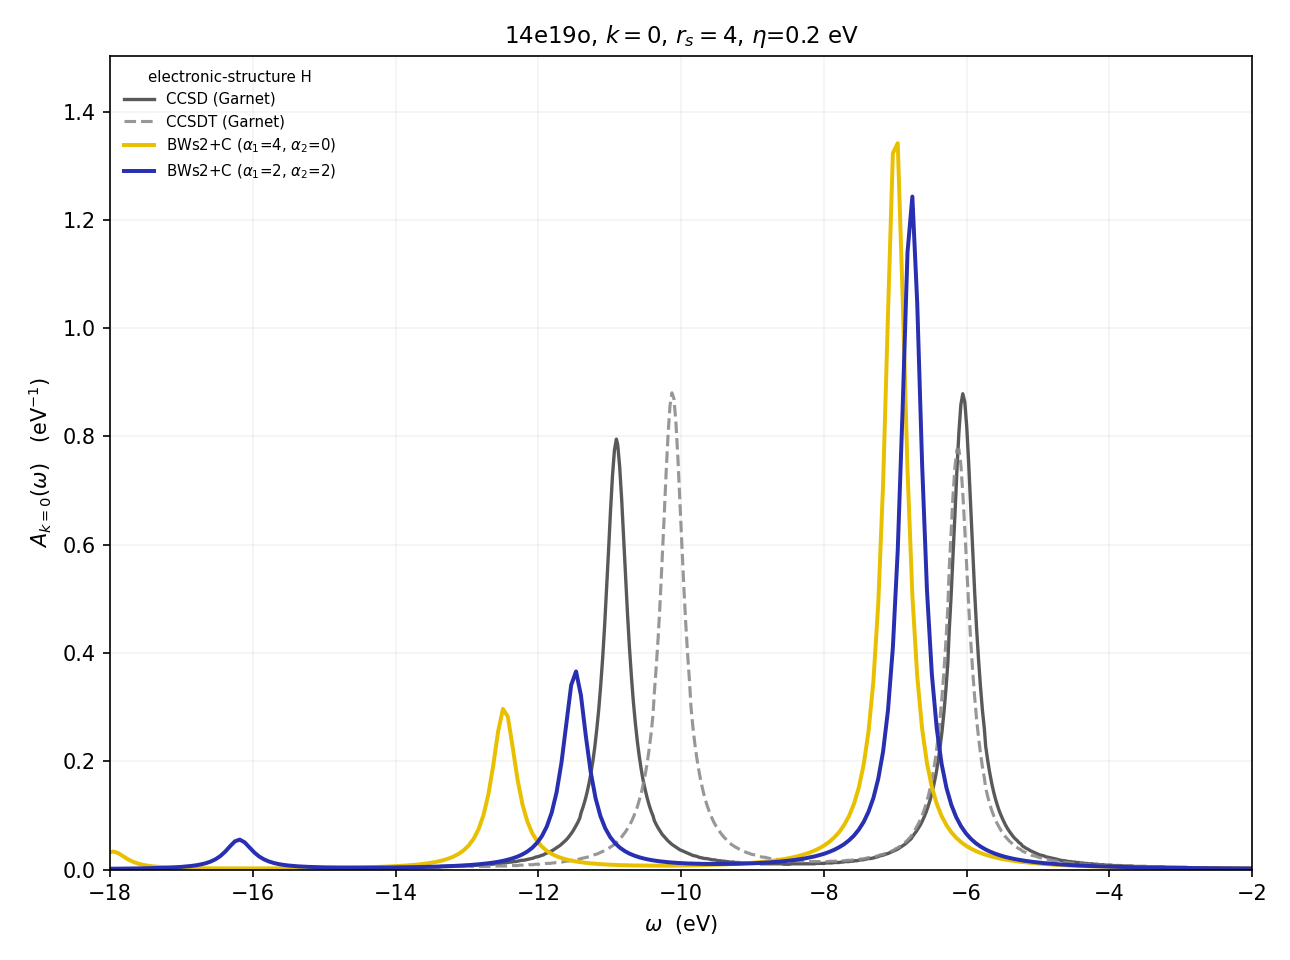
\includegraphics[width=0.8\textwidth]{26/9/9-23/k0_14e19o_single_panel_bws2.png}
\end{figure}
\end{frame}
\begin{frame}
    \frametitle{BW ES curves for 114e485o}
    \begin{figure}
        \centering
        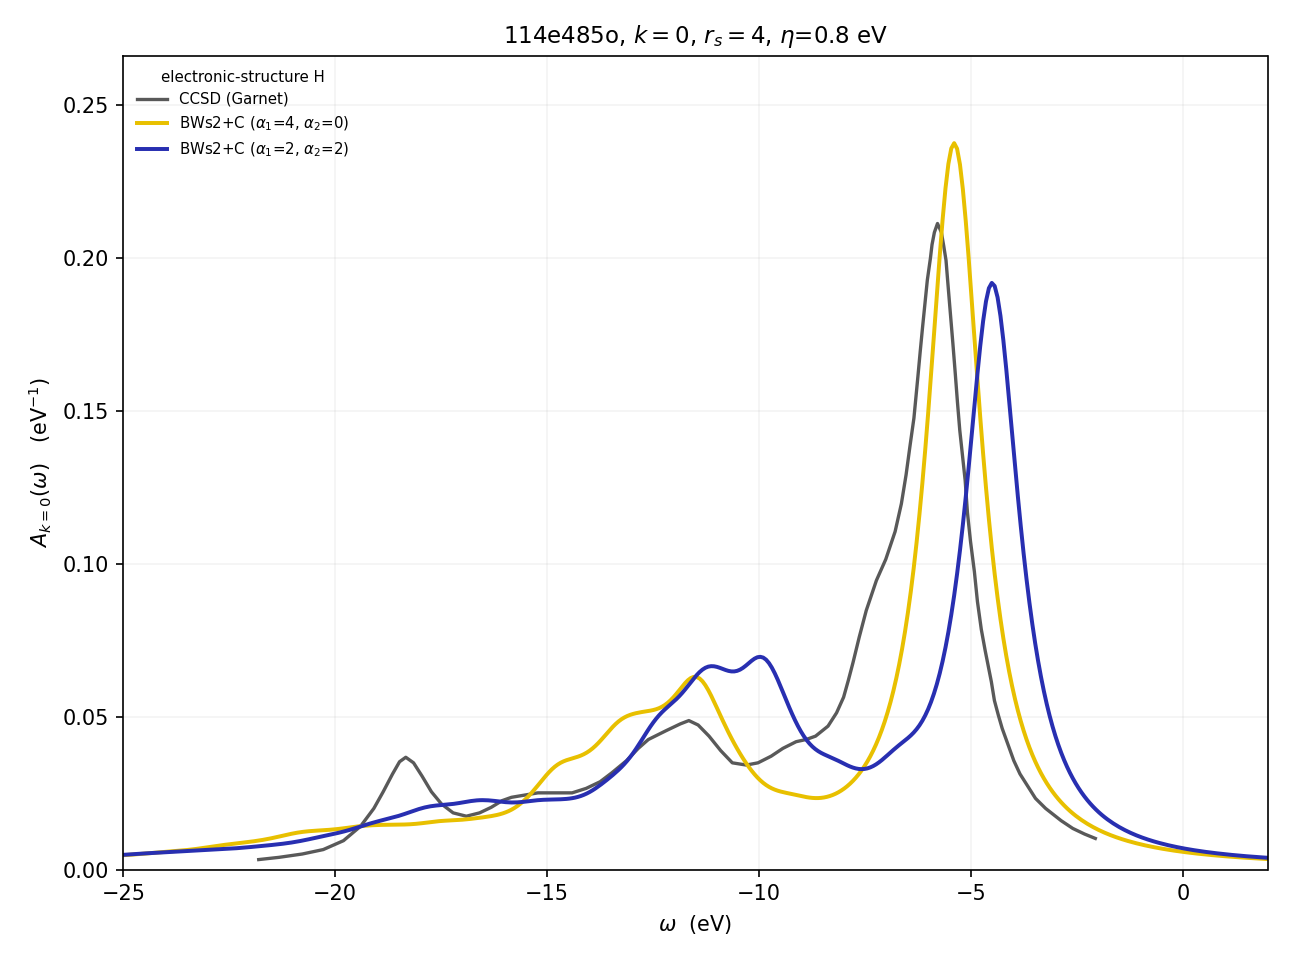
\includegraphics[width=0.8\textwidth]{26/9/9-23/k0_114e485o_single_panel_bws2.png}
\end{figure}
\end{frame}
\begin{frame}
    \frametitle{Partitioning }
 The BWs2 partition chooses
\begin{equation}
    \hat{H} = \hat{H}_0' + \hat{H}_1',
\end{equation}
with
\begin{equation}
\mathbf{H}_0' = \begin{pmatrix} \mathbf{F}_{oo} + \alpha_1 \mathbf{W}^{O} & 0 \\ 0 & \mathbf{F}_{vv} + \alpha_2 \mathbf{W}^{V} \end{pmatrix},
\end{equation}\pause
where we assume a canonical Hartree-Fock matrix and define 
\begin{align}
{W}^{O}_{ii} &= \frac{1}{2}\bm{\Sigma}_{ii}^{(2),2p1h}(\omega = \tilde{\varepsilon}_i)= \frac{1}{2}\sum_{a b j} \frac{\mathcal{K}_{ij}^{ab}}{\tilde{\varepsilon}_i + \tilde{\varepsilon}_j - \tilde{\varepsilon}_a - \tilde{\varepsilon}_b},\\
\mathbf{W}^{V}_{aa} &= \frac{1}{2}\bm{\Sigma}_{aa}^{(2),2h1p}(\omega = \tilde{\varepsilon}_a)= \frac{1}{2}\sum_{i j b} \frac{\mathcal{K}_{ij}^{ab}}{\tilde{\varepsilon}_a + \tilde{\varepsilon}_b - \tilde{\varepsilon}_i - \tilde{\varepsilon}_j},
\end{align}\pause
where $\tilde{\varepsilon}$ is the BWs2 ground-state MO energy and we defined $\mathcal K_{pq}^{rs} =
(pr|qs)
\left[
2(pr|qs)-(ps|qr)
\right]$.
 \pause \textbf{Bug 1} In the spin-restricted formalism, we must have $\operatorname{Tr}(\alpha_1\mathbf{W}^{O}) = \frac{\alpha_1}{2}E_{\text{MP2}}$. 
\end{frame}
\begin{frame}
    \frametitle{Defining the cumulant }
We define the noninteracting Green's function as
\begin{equation}
G^{(0)'}(\omega)
=
\big( \omega - (\mathbf{F} + \underbrace{\alpha_1 \mathbf{W}^O \oplus \alpha_2 \mathbf{W}^V}_{\mathbf{W}}) \big)^{-1}.
\end{equation}\pause
The Dyson equation becomes
\begin{align}
G^{-1}(\omega)
% &= \omega - \mathbf{F} - \bm{\Sigma}(\omega) \\
&= \omega - (\mathbf{F} + \mathbf{W})
   - \big[ \bm{\Sigma}(\omega) - \mathbf{W} \big] \\
&= \big( G^{(0)'}(\omega) \big)^{-1}
   - \bm{\Sigma}_{\mathrm{eff}}(\omega).
\end{align}\pause
Setting Dyson and cumulant expansions for the hole state $p$ equal to 2nd order in $v$
implies
\begin{align}
C_{pp}^{\mathrm{BWs2}}(t)
% &=
% i \int \frac{d\omega}{2\pi}
% e^{-i(\omega - \tilde{\varepsilon}_p)t}
% \frac{\Sigma_{\mathrm{eff},pp}(\omega)}
%      {(\omega - \tilde{\varepsilon}_p)^2} \\
&=
i \int \frac{d\omega'}{2\pi}
e^{-i\omega' t}
\frac{\Sigma_{\mathrm{eff},pp}(\omega' + \tilde{\varepsilon}_p)}
     {(\omega')^2}. %\\
% &=
% \int d\omega\,
% \frac{\beta_{pp}(\omega)}{\omega^2}
% \left(
% e^{-i \omega t}
% + i \omega t
% - 1
% \right),
\end{align}\pause
with $\Sigma_{\mathrm{eff},pp}(\omega) = \Sigma_{pp}[G^{(0)'}](\omega) -W_{pp}$. \pause \textbf{Bug 2} It should be $W_{pp}=\alpha_1 W^{O}_{pp}$, but I had $W_{pp}=\alpha_1 W^{O}_{pp} + \alpha_2 W^{V}_{pp}$.
\end{frame}
\begin{frame}
    \frametitle{Ideas for what to try next }
\begin{itemize}
    \item These are the only regularization parameters we are interested in moving forward? \pause
    \item Nemo thinks that 2,2 should converge to 4,0 as we expand the virtual space \end{itemize}
\end{frame}
\section{What is the quasiboson Hamiltonian?}
\begin{frame}
    \frametitle{Formal definitions}
\begin{align}
\hat{H}
&=
\hat{H}_{\rm el}
+
\hat{H}_{\rm pl}
+
\hat{H}_{\rm ep}
\\
&=
\sum_{\bm{k}\in\mathcal{O}}
\epsilon_{\bm{k}}^{\rm G0}
h_{\bm{k}}^{\dagger}h_{\bm{k}}
+
\sum_{\nu_{\bm{q}}\in\mathcal{M}}
\omega_{\nu_{\bm{q}}}^{\rm pl}
b_{\nu_{\bm{q}}}^{\dagger}
b_{\nu_{\bm{q}}}
\nonumber\\
&\quad
+
\sum_{\bm{k},\bm{k}+\bm{q}\in\mathcal{O}}
\sum_{\nu_{\bm{q}}\in\mathcal{M}}
g_{\nu}^{\rm pl}(\bm{k},\bm{q})
h_{\bm{k}+\bm{q}}^{\dagger}
h_{\bm{k}}
\left(
b_{\nu_{-\bm{q}}}^{\dagger}
+
b_{\nu_{\bm{q}}}
\right).
\label{eq:H}
\end{align}\pause
Dunn's SC-CE solves
\begin{align}
\frac{dC_{\bm{k}}(t)}{dt}
&=
-i\Delta_{\bm{k}}^x
-
\sum_{\nu_{\bm q}}
\left|g_\nu^{\rm pl}(\bm{k},\bm q)\right|^2
\int_0^t d\tau\,
e^{i\Delta_{\bm{k}\bm q}^{\nu}(t-\tau)}
e^{
-C_{\bm{k}}(t)+C_{\bm{k}}(\tau)
+C_{\bm{k}-\bm q}(t)-C_{\bm{k}-\bm q}(\tau)
}.
\end{align}\pause
To recover $G_0W_0$+C, set all $C_{\bm{k}}(t)=0$ in the memory kernel
\end{frame}
\begin{frame}
    \frametitle{GW ES curves for 14e19o}
    \begin{figure}
        \centering
        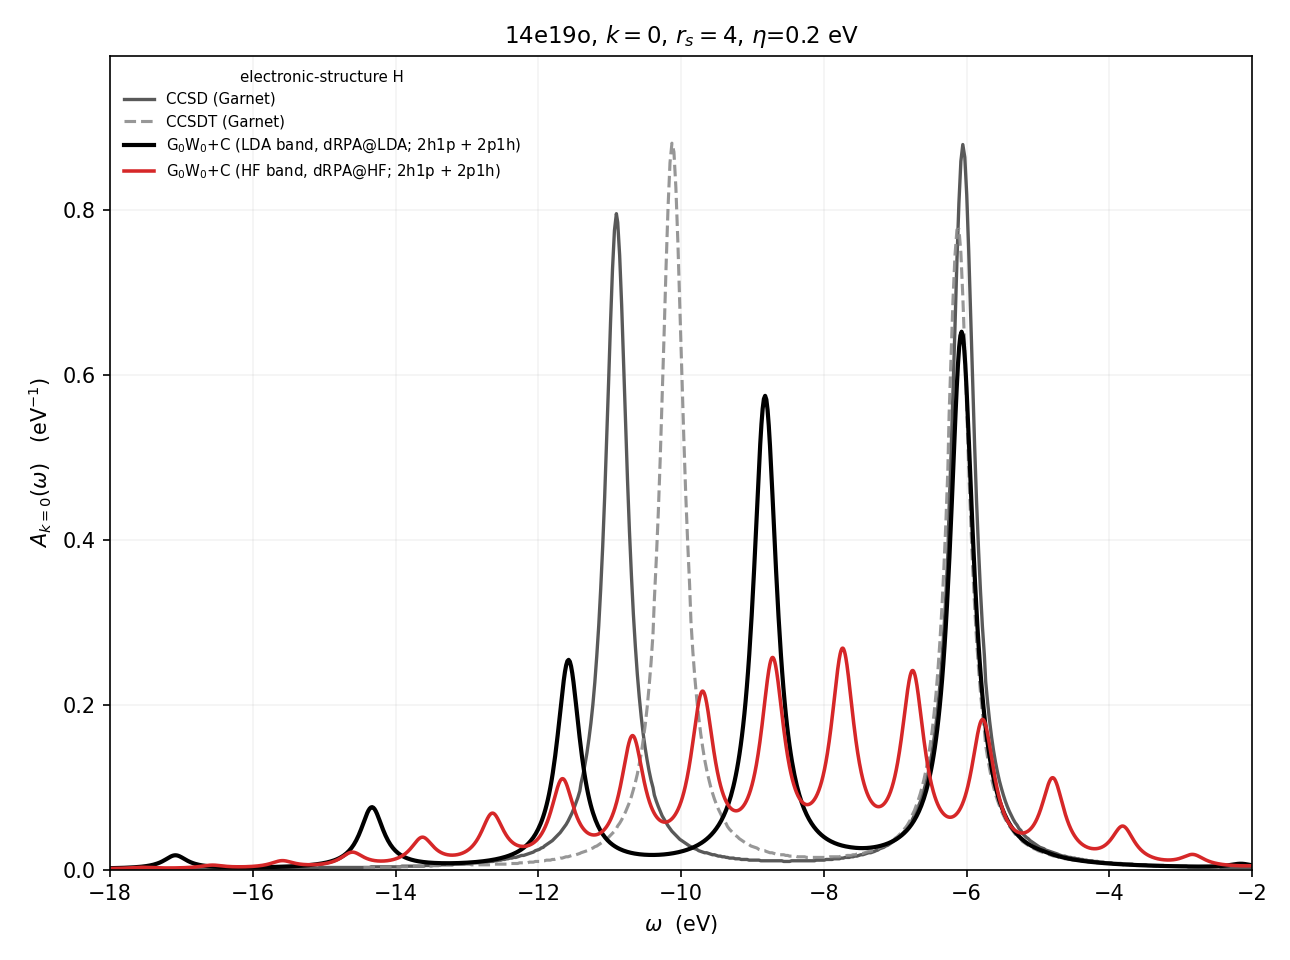
\includegraphics[width=0.8\textwidth]{26/9/9-23/k0_14e19o_single_panel_g0w0c.png}
\end{figure}
\end{frame}
\begin{frame}
    \frametitle{GW ES+QB curves for 14e19o}
    \begin{figure}
        \centering
        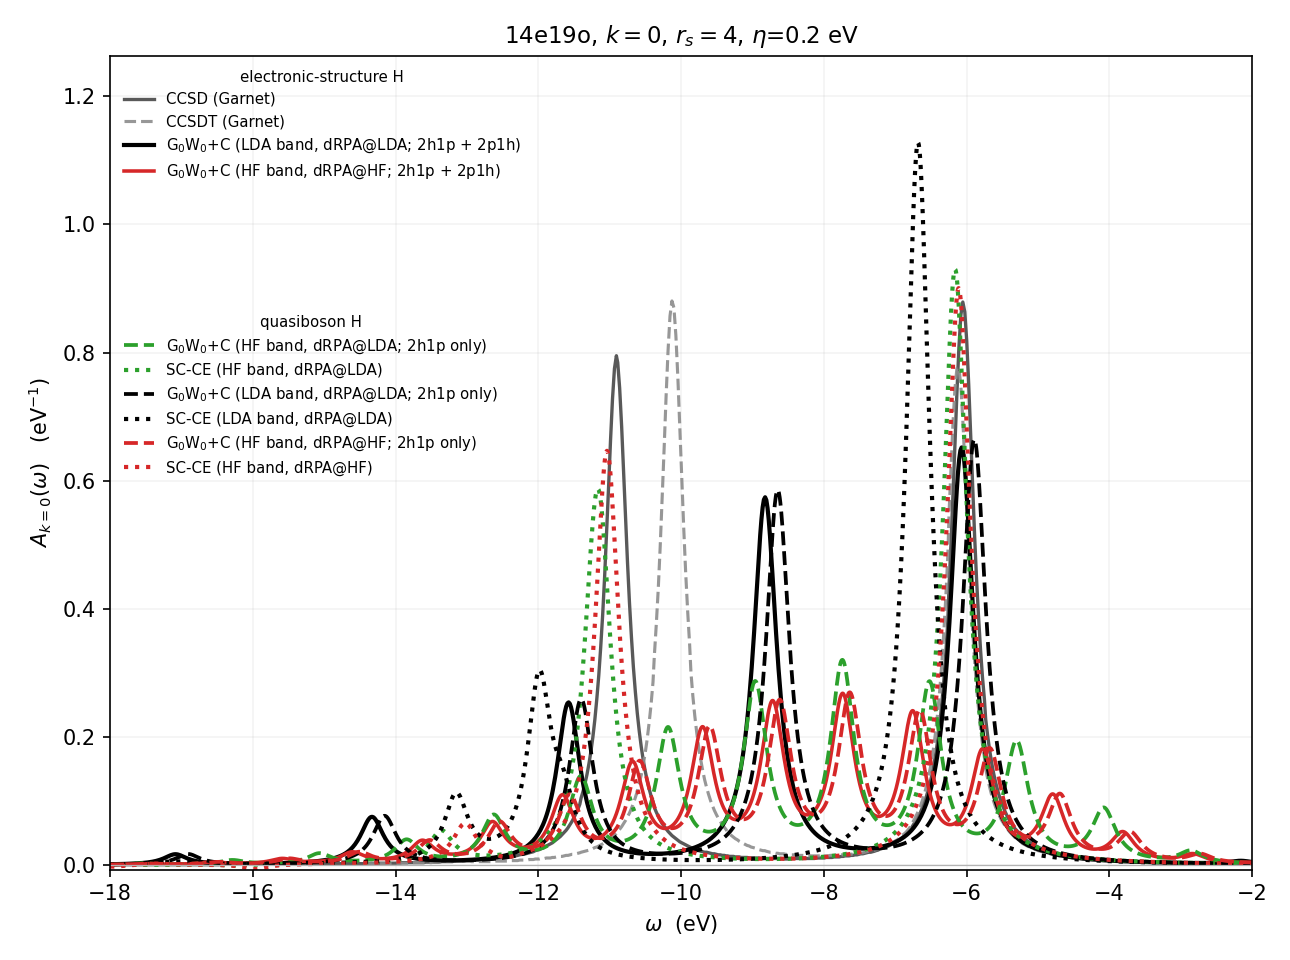
\includegraphics[width=0.8\textwidth]{26/9/9-23/k0_14e19o_single_panel_qb.png}
\end{figure}
\end{frame}
\begin{frame}
    \frametitle{GW ES curves for 114e485o}
    \begin{figure}
        \centering
        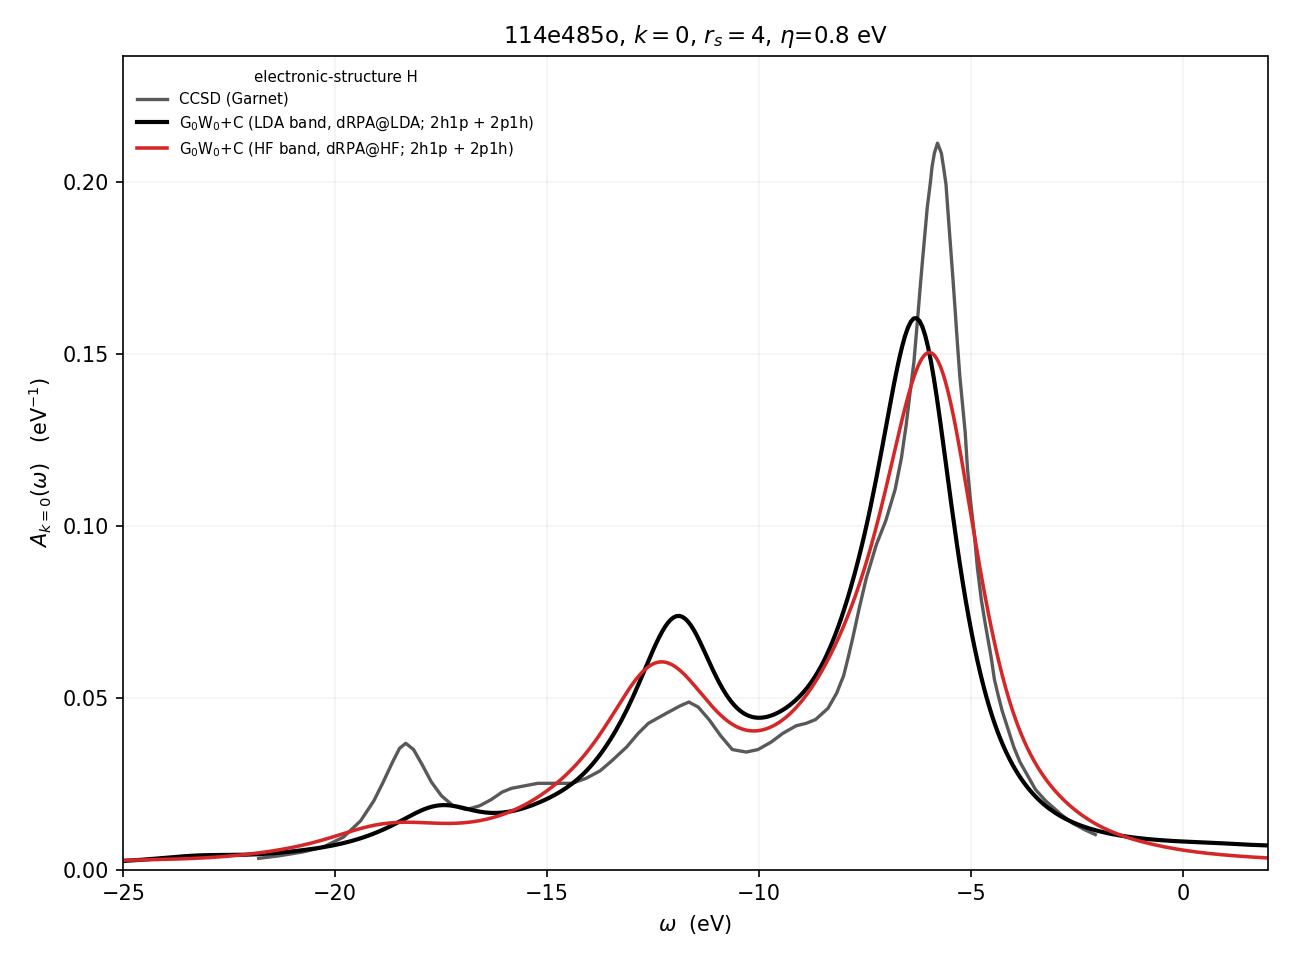
\includegraphics[width=0.8\textwidth]{26/9/9-23/k0_114e485o_single_panel_g0w0c.png}
\end{figure}
\end{frame}
\begin{frame}
    \frametitle{GW ES+QB curves for 114e485o}
    \begin{figure}
        \centering
        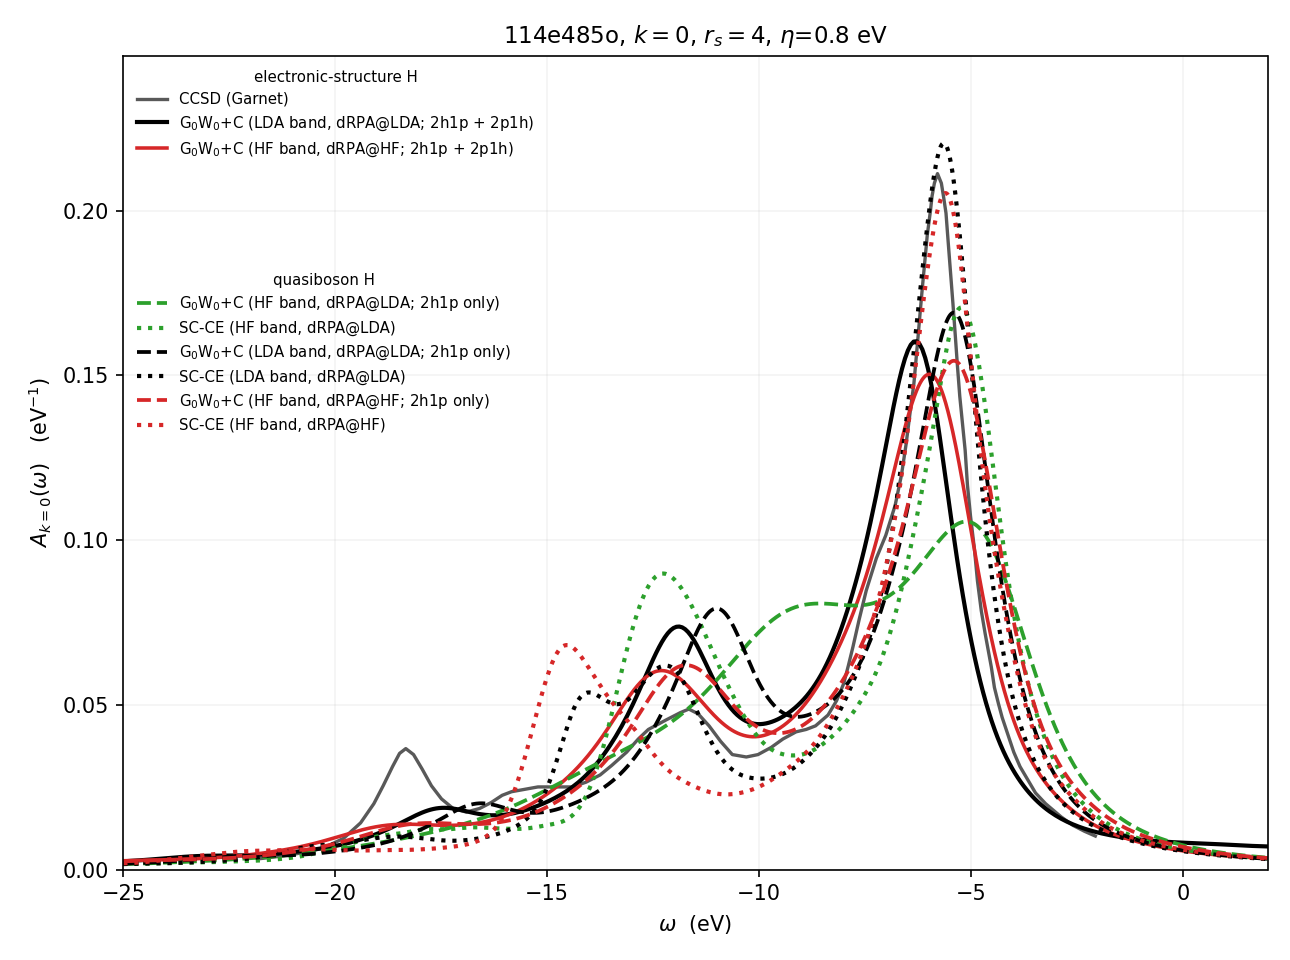
\includegraphics[width=0.8\textwidth]{26/9/9-23/k0_114e485o_single_panel_qb.png}
\end{figure}
\end{frame}

\begin{frame}
    \frametitle{Variants explored}
\textbf{LDA band, dRPA@LDA plasmons}\\
$\Delta_{\bm{k}\bm q}^{\nu}
\equiv
\epsilon_{\bm{k}}^{\rm LDA}
-\epsilon_{\bm{k}-\bm q}^{\rm LDA}
+\omega_{\nu_{\bm q}}^{\rm pl}$ and $\Delta_{\bm{k}}^x\equiv -n_{\bm k}v_m-\sum_{\bm q\neq\bm 0}n_{\bm k+\bm q}v(\bm q)-V_{x c, k}^{\mathrm{LDA}}$. \pause The plasmonic bath is due to dRPA@LDA, so our Casida build uses $A_{ia,jb}(\mathbf{q}) = \delta_{ij} \delta_{ab} (\epsilon_a^{\rm LDA} - \epsilon_i^{\rm LDA}) + 2 (ia|bj)$ and $B_{ia,jb}(\mathbf{q}) = 2 (ia|jb)$. \pause This is what I have been showing for G0W0+C. \\ \pause
\textbf{HF band, dRPA@HF plasmons}\\
$\Delta_{\bm{k}\bm q}^{\nu}
\equiv
\epsilon_{\bm{k}}^{\rm HF}
-\epsilon_{\bm{k}-\bm q}^{\rm HF}
+\omega_{\nu_{\bm q}}^{\rm pl}$ and $\Delta_{\bm{k}}^x\equiv 0$. \pause The plasmonic bath is due to dRPA@HF, so our Casida build uses $A_{ia,jb}(\mathbf{q}) = \delta_{ij} \delta_{ab} (\varepsilon_a^{\rm HF} - \varepsilon_i^{\rm HF}) + 2 (ia|bj)$ and $B_{ia,jb}(\mathbf{q}) = 2 (ia|jb)$. \pause $\varepsilon_k^{\rm HF}\equiv k^2/2 -\sum_{\bm{q}\neq\bm{0}} n_{\bm{k}+\bm{q}} v(\bm{q})$ and $\epsilon_k^{\rm HF} = k^2/2 - n_{k}v_m-\sum_{\bm{q}\neq\bm{0}} n_{\bm{k}+\bm{q}}v(\bm{q})$.\\ \pause
\textbf{HF band, dRPA@LDA plasmons}\\
$\Delta_{\bm{k}\bm q}^{\nu}
\equiv
\epsilon_{\bm{k}}^{\rm HF}
-\epsilon_{\bm{k}-\bm q}^{\rm HF}
+\omega_{\nu_{\bm q}}^{\rm pl}$ and $\Delta_{\bm{k}}^x\equiv 0$. \pause The plasmonic bath is due to dRPA@LDA, so our Casida build uses $A_{ia,jb}(\mathbf{q}) = \delta_{ij} \delta_{ab} (\varepsilon_a^{\rm LDA} - \varepsilon_i^{\rm LDA}) + 2 (ia|bj)$ and $B_{ia,jb}(\mathbf{q}) = 2 (ia|jb)$.
\end{frame}
\begin{frame}
    \frametitle{Why dRPA@HF doesn't look so different}
We redefined the Hamiltonian with shifted Ewald summation. \pause Madelung potential is a correction for a spurious interaction of image charges in periodic simulation. \pause But dRPA computes neutral excitation energies, so it shouldn't see image charges. \pause This is why when the plasmonic bath is due to dRPA@HF, our Casida build should use $A_{ia,jb}(\mathbf{q}) = \delta_{ij} \delta_{ab} (\varepsilon_a^{\rm HF} - \varepsilon_i^{\rm HF}) + 2 (ia|bj)$ and $B_{ia,jb}(\mathbf{q}) = 2 (ia|jb)$ where $\varepsilon_k^{\rm HF}\equiv k^2/2 -\sum_{\bm{q}\neq\bm{0}} n_{\bm{k}+\bm{q}} v(\bm{q})$. \pause Garnet used $\epsilon^{\rm HF}$ to compute dRPA@HF, which is why GW@HF looked bad in his study. \pause Does it mean he made an error, did I make an error, or does it mean that a non-local reference should not be used for periodic GW simulations? \pause Does this have anything to do with the slow basis set convergence of abG0W0 or no?
\end{frame}
\section{All the results}
\begin{frame}
    \frametitle{Everything for 14e19o}
    \begin{figure}
        \centering
        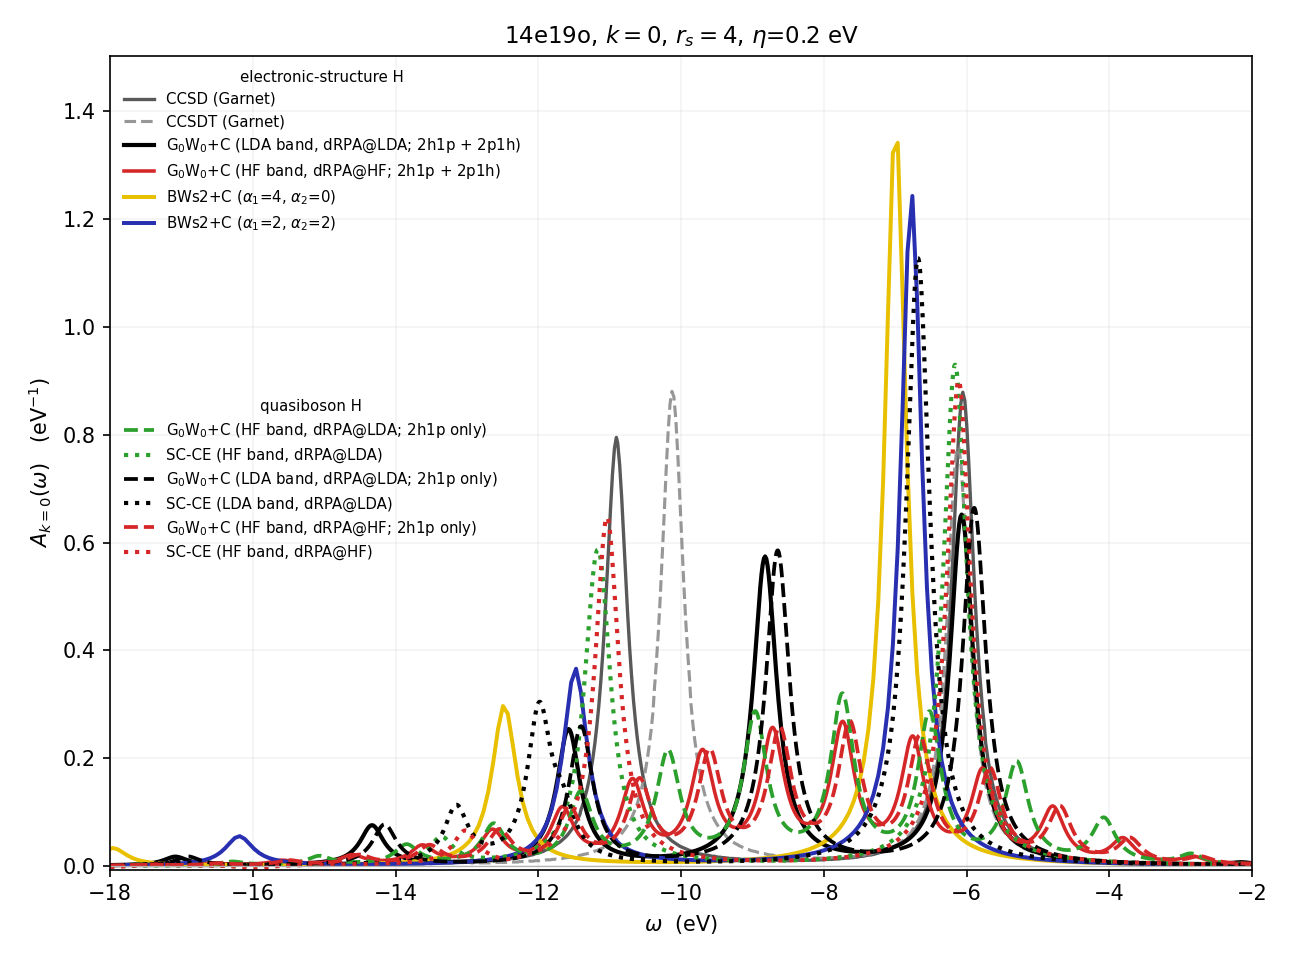
\includegraphics[width=0.8\textwidth]{26/9/9-23/k0_14e19o_single_panel.png}
\end{figure}
\end{frame}
\begin{frame}
    \frametitle{Everything for 114e485o}
    \begin{figure}
        \centering
        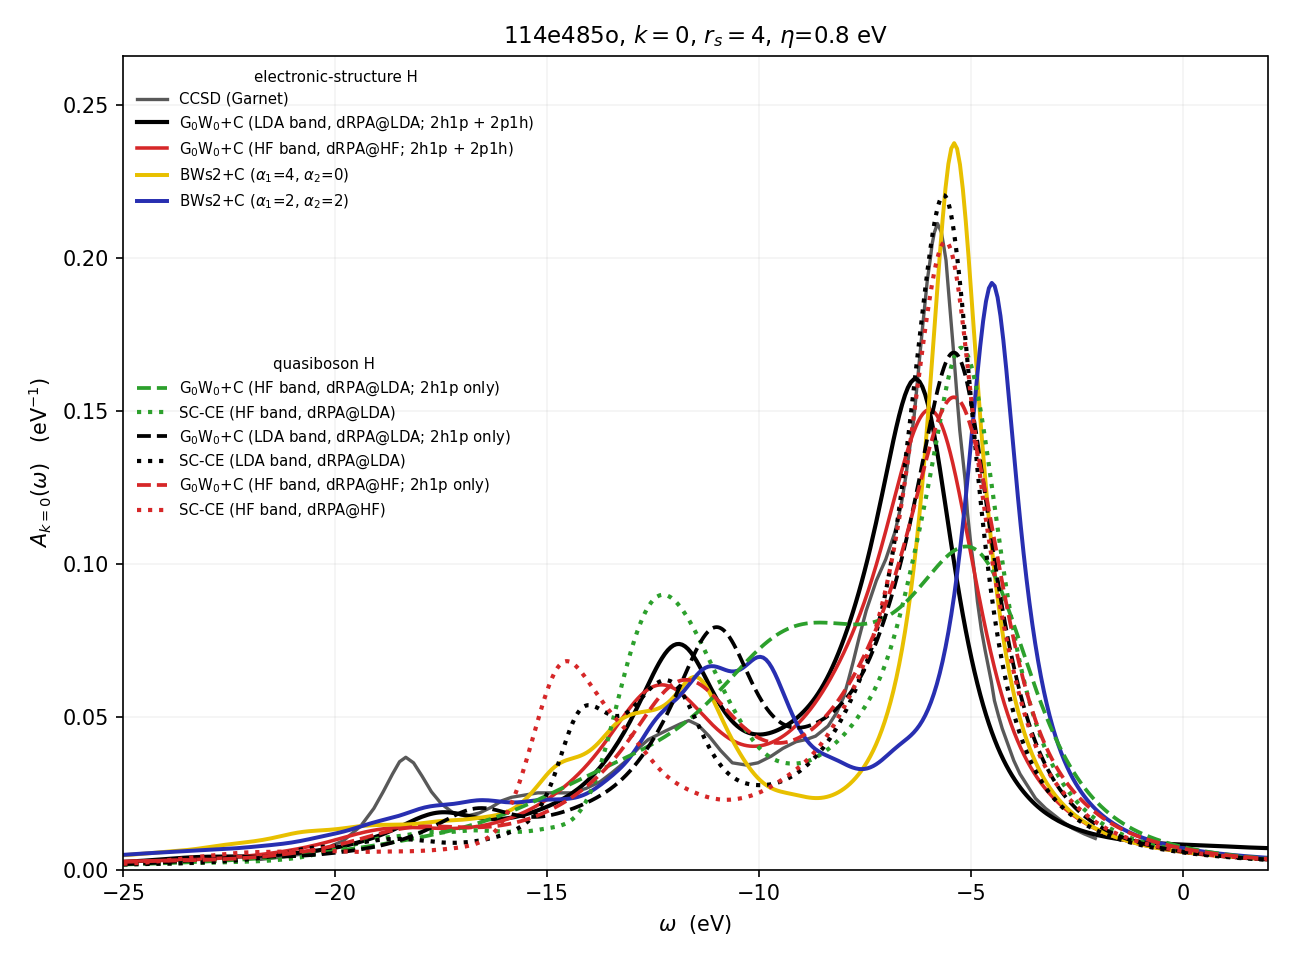
\includegraphics[width=0.8\textwidth]{26/9/9-23/k0_114e485o_single_panel.png}
\end{figure}
\end{frame}
\section{Derivation of fermionic cumulants}
\begin{frame}
    \frametitle{Partitioning}
Define the static BWs2 shift as
\begin{equation}
\Lambda_p
=
\begin{cases}
\alpha_1 W_p^{O}, & p\in\mathcal O,\\[1mm]
\alpha_2 W_p^{V}, & p\in\mathcal V,
\end{cases}
\qquad
\tilde{\epsilon}_p
=
\epsilon_p+\Lambda_p.
\end{equation}
The Hamiltonian is partitioned as
\begin{align}
\hat H
&=
\hat H_0^{\rm BW}
+
\hat V^{\rm BW},\\
\hat H_0^{\rm BW}
&=
\sum_p
\tilde{\epsilon}_p\hat n_p,\\
\hat V^{\rm BW}
&=
\hat V
-
\sum_p
\Lambda_p\hat n_p .
\end{align}
% Introducing the auxiliary phases $\phi_p(t)$ gives
% \begin{align}
% \hat H_0^{{\rm BW},\phi}(t)
% &=
% \hat H_0^{\rm BW}
% +
% \sum_p\dot{\phi}_p(t)\hat n_p,\\
% \hat V^{{\rm BW},\phi}(t)
% &=
% \hat V
% -
% \sum_p\Lambda_p\hat n_p
% -
% \sum_p\dot{\phi}_p(t)\hat n_p .
% \end{align}
% Counting $
% \hat V=\mathcal O(\lambda)$, $
% \Lambda_p=\mathcal O(\lambda^2)$, and $
% \phi_p=\mathcal O(\lambda^2)$, suggests that we can treat the BWs2 and auxiliary one-body counterterms the same way. So after the cancellation of the explicit auxiliary phase, we have
% \begin{align}
% C_c^+(t)
% &=
% +i\Lambda_c t
% +
% \left[\ln y_c^\phi(t)\right]_{WW}^{(2)},\\
% C_k^-(t)
% &=
% -i\Lambda_k t
% +
% \left[\ln y_k^\phi(t)\right]_{WW}^{(2)}.
% \end{align}
\end{frame}
\begin{frame}
    \frametitle{End result}
Thus, the end result for the coupled VIDEs
\begin{align}
\dot C_c^+(t)
&=
+i\Lambda_c
-
\sum_{iab}
\mathcal{K}_{ci}^{ab}
\int_0^t d\tau\,
e^{-i\widetilde{\Delta}_{cabi}^{(+)}(t-\tau)}
\nonumber\\
&\qquad\times
\exp\left[
-\delta C_c^+
+\delta C_a^+
+\delta C_b^+
+\delta C_i^-
\right],
\\[2mm]
\dot C_k^-(t)
&=
-i\Lambda_k
+
\sum_{ija}
\mathcal{K}_{ij}^{pa}
\int_0^t d\tau\,
e^{-i\widetilde{\Delta}_{kija}^{(-)}(t-\tau)}
\nonumber\\
&\qquad\times
\exp\left[
-\delta C_k^-
+\delta C_i^-
+\delta C_j^-
+\delta C_a^+
\right],
\end{align}
with $\delta C_q\equiv C_q(t)-C_q(\tau)$, $\widetilde{\Delta}_{cabi}^{(+)}=\tilde{\epsilon}_a+\tilde{\epsilon}_b-\tilde{\epsilon}_c-\tilde{\epsilon}_i$, and $\widetilde{\Delta}_{kija}^{(-)}=\tilde{\epsilon}_k+\tilde{\epsilon}_a-\tilde{\epsilon}_i-\tilde{\epsilon}_j$.
\pause Need to solve these ODEs simultaneously.
\end{frame}